\begin{question}{30}{
    In een gezamenlijk project van sportinstructeurs van de KMA en de geneeskundige dienst wordt het verband onderzocht tussen de gemiddelde slaaptijd van een cadet (in uren) en de hersteltijd na een zware inspanning (in uren).
    Voor de hersteltijd wordt gekeken naar een spierpijn-index, en een cadet is volledig hersteld wanneer de spierpijn-index onder een gegeven drempelwaarde komt.

    Van negen cadetten wordt gemeten hoe lang ze gemiddeld hebben geslapen en hoe lang hun hersteltijd is na een zware inspanning.
    \begin{center}
        \begin{tabular}{c|ccccccccc}
            \toprule
                \textbf{Slaaptijd (in uren)} & $4,0$ & $4,5$ & $5,0$ & $5,5$ & $6,0$ & $6,5$ & $7,0$ & $7,5$ & $8,0$ \\
                \textbf{Hersteltijd na zware inspanning (in uren)} & $66$ & $61$ & $63$ & $62$ & $65$ & $64$ & $57$ & $59$ & $60$ \\
            \bottomrule
        \end{tabular}
    \end{center}
}
    \subquestion{2}{
        Als we een regressie-analyse willen uitvoeren, welke variabele zou dan de afhankelijke variabele $Y$ zijn en welke variabele zou de onafhankelijke variabele $X$ zijn?
    }
    \solution{
        Bij een regressie-analyse is de meest logische keuze om slaaptijd als onafhankelijke variabele $X$ te kiezen, en de hersteltijd als afhankelijke variabele $Y$. 
        Een langere hersteltijd verklaart niet waarom iemand langer slaapt, terwijl dat andersom wellicht wel het geval kan zijn.
    }
    \subquestion{5}{
        Teken het bijbehorende spreidingsdiagram op basis van je antwoord op vraag (a).
    }
    \solution{
        \begin{center}
            \resizebox{0.9\textwidth}{!}{
                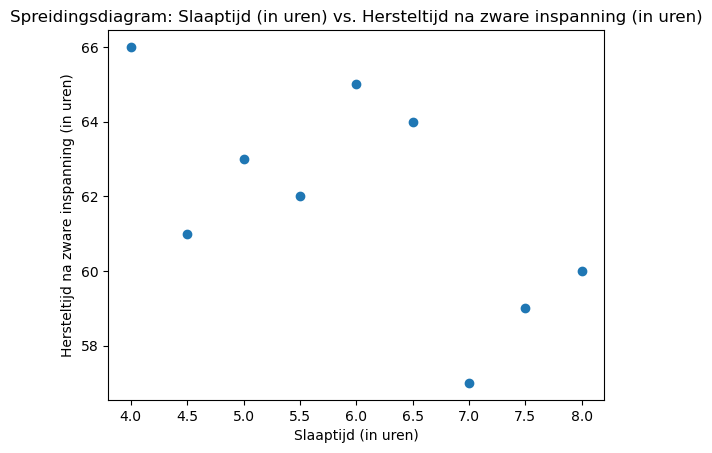
\includegraphics{20250725_q4_scatterplot.png}
            }
        \end{center}
    }

    \subquestion{8}{
        Bereken Pearson's correlatieco\"effici\"ent $r(x,y)$.
        Wat kun je concluderen over de samenhang van de twee variabelen?
    }
    \solution{
        We beginnen met het uitrekenen van Pearson's correlatieco\"effici\"ent 
        \begin{align*}
            r(x, y) = \frac{\overline{xy} - \overline{x} \cdot \overline{y}}{\sqrt{(\overline{x^2} - \overline{x}^2)\cdot(\overline{y^2} - \overline{y}^2) }}
        \end{align*}
        Hiervoor hebben we dus de waardes van $\overline{x}$, $\overline{y}$, $\overline{xy}$, $\overline{x^2}$ en $\overline{y^2}$ nodig.
        Deze bepalen we aan de hand van de volgende rekentabel:
        \begin{center}
            \begin{tabular}{ccccc}
                \toprule
                    $x$ & $y$ & $xy$ & $x^2$ & $y^2$ \\
                \midrule
    		        $4$ & $66$ & $264$ & $16$ & $4356$ \\
                    $4,5$ & $61$ & $274,5$ & $20,25$ & $3721$ \\
                    $5$ & $63$ & $315$ & $25$ & $3969$ \\
                    $5,5$ & $62$ & $341$ & $30,25$ & $3844$ \\
                    $6$ & $65$ & $390$ & $36$ & $4225$ \\
                    $6,5$ & $64$ & $416$ & $42,25$ & $4096$ \\
                    $7$ & $57$ & $399$ & $49$ & $3249$ \\
                    $7,5$ & $59$ & $442,5$ & $56,25$ & $3481$ \\
                    $8$ & $60$ & $480$ & $64$ & $3600$ \\
                \midrule
                    $\overline{x} = 6$ & $\overline{y} = 61,8889$ & $\overline{xy} = 369,1111$ & $\overline{x^2} = 37,6667$ & $\overline{y^2} = 3837,8889$ \\
                \bottomrule
            \end{tabular} \rubric{4}
        \end{center}
        De correlatieco\"effici\"ent van Pearson is dus gelijk aan
        \begin{align*}
            r(x,y)  &= \frac{ \overline{x \cdot y} - \overline{x} \cdot \overline{y} }{ \sqrt{ (\overline{x}^2 - \overline{x^2}) \cdot (\overline{y}^2 - \overline{y^2}) } }\\
                    &= \frac{ 369,1111 - 6 \cdot 61,8889 }{ \sqrt{ (6^2 - 37,6667) \cdot (61,8889^2 - 3837,8889) } } \\
                    &= \frac{-2,2222}{3,5717} \\
                    &\approx -0,6222.\rubric{3}
        \end{align*}
        De correlatieco\"effici\"ent ligt redelijk ver van 0 en is negatief.
        Dit houdt in dat er een vrij duidelijke dalende trend zichtbaar is, maar dat er toch onzekerheid zit in hoe het exacte lineaire verband eruit zal zien. \rubric{1}
    }

    \subquestion{7}{
        Bereken de regressielijn $Y = a + b \cdot X$ door berekening van de co\"effici\"enten $a$ en $b$.
        Bepaal aan de hand van de regressielijn een statistisch verantwoorde voorspelling voor de hersteltijd van een cadet die gemiddelde $6$ uur en $45$ minuten heeft geslapen.
    }
    \solution{
        Om de co\"effici\"enten $a$ en $b$ van de regressielijn te berekenen, gaan we de rekentabel van vraag (a) hergebruiken.
        Er volgt namelijk dat
        \begin{align*}
            b &= \frac{\overline{xy} - \overline{x} \cdot \overline{y}}{\overline{x^2} - (\overline{x})^2} \\
              &= \frac{369,1111 - 6 \cdot 61,8889}{37,6667 - (6)^2} \\
              &= \frac{-2,2222}{1,6667} \approx -1,3333 \\ \rubric{2}
            a &= \overline{y} - b \cdot \overline{x} \\
              &= 61,8889 - -1,3333 \cdot 6 \\ 
              &\approx 69,8889.\rubric{2}
        \end{align*}
        De formule van de regressielijn is dus gelijk aan $Y = 69,8889 - 1,3333 \cdot X$. \rubric{1}
        Een statistisch verantwoorde voorspelling voor de hersteltijd van een cadet die gemiddelde $6$ uur en $45$ minuten heeft geslapen vinden we door $X = 6,75$ in te vullen:
        Dit geeft een waarde van $Y = 69,8889 - 1,3333 \cdot 6,75 = 60,88887$ uur, oftewel iets minder dan $61$ uur. \rubric{2} 
    }

    \subquestion{8}{
        Bereken een $90\%$-voorspellingsinterval voor de hersteltijd van een willekeurige cadet die $6$ uur en $45$ minuten heeft geslapen.
    }
    \solution{
        DIn opdracht (d) hebben we een puntschatting van $y_0 = 69,8889 -1,3333 \cdot 6,75 \approx 60,8889$ bepaald.
        Daarnaast kunnen we de standaardafwijking $\sigma$ van de storingsterm $\varepsilon$ schatten:
        \begin{align*}
            s_{\varepsilon} &= \sqrt{ \frac{n}{n-2} \cdot \left( \overline{y^2} - a \cdot \overline{y} - b \cdot \overline{xy} \right) } \\ 
                               &= \sqrt{ \frac{9}{7} \cdot \left( 3837,8889 - 69,8889 \cdot 61,8889 - -1,3333 \cdot 369,1111 \right) } \\ 
                               &\approx 2,456. \rubric{3}
        \end{align*}

        Vervolgens kunnen we een puntschatting berekenen van de standaardafwijking van $Y$ voor gegeven $X = x_0$:
        \begin{align*}
            s_{f} &= s_{\varepsilon} \cdot \sqrt{ 1 + \frac{1}{n} \cdot \left( 1 + \frac{(x_0 - \overline{x})^2}{\overline{x^2} - \overline{x}^2} \right) } \\
                    &= 2,456 \cdot \sqrt{ 1 + \frac{1}{9} \cdot \left( 1 + \frac{(6,75 - 6)^2}{37,6667 - 6^2} \right) } \\
                    &\approx 2,6321.  \rubric{2}       
        \end{align*}

        Omdat we de standaardafwijkingen geschat hebben en de storingstermen normaal verdeeld zijn, moeten we werken met de $t$-verdeling met $df = n - 2 = 7$ vrijheidsgraden.
        De $t$-waarde die hoort bij een betrouwbaarheidsniveau $\alpha = 0,1$ is gelijk aan
        \[
            t = \invt(\text{opp} = 1 - \alpha / 2; \text{df} = n - 2) = \invt(\text{opp} = 0,95; \text{df} = 7) \approx 1,8946. \rubric{1}
        \]
        Het \SI{90}{\percent}-betrouwbaarheidsinterval voor de gemiddelde $Y$ voor gegeven $X = x_0$ kan dus worden beschreven door
        \begin{align*}
            &[y_0 - t \cdot s_{f}; y_0 - t \cdot s_{f}] \\ 
            &= [60,8889 - 1,8946 \cdot 2,6321; 60,8889 + 1,8946 \cdot 2,6321] \\ 
            &\approx [55,9021; 65,8757]. \rubric{2}
        \end{align*}
        
        Met \SI{90}{\percent} betrouwbaarheid ligt een toekomstige uitkomst van $Y$ voor gegeven $X = 6,75$ tussen $55,9021$ en $65,8757$.
    }
\end{question}